
%% Title Page 
\title{\Huge Functional Requirements Document Spesification \\ 
	 Project: \\ 
	Cafeteria Management System: Reslove}
\author{
         \underline{T-RISE}\\
          Rendani Dau (13381467) \\
	Elana Kuun (12029522) \\
	Semaka Malapane (13081129) \\
	Antonia Michael (13014171) \\
	Isabel Nel (13070305)}
\\
\url{https://github.com/toniamichael94/MainProjectCOS301}
\\
\date{\today}

\documentclass[12pt]{article}

\begin{document}
\maketitle
\break

%% Make table of contents
\tableofcontents
\break

%%now begin document

%%---------------------------------  INTRODUCTION -------------------------------------------
\section{Introduction}
This document contains the functional requirements specification, architecture requirements and testing for the Resolve Cafeteria Management System that will be created for Software Engineering (COS 301) at the University of Pretoria 2015, by the group T-RISE. In this document we will thoroughly discuss and layout the project's architectural requirements , functional requirements, application design and testing to provide a clear view of the system as a whole. An agile approach is being followed, hence the main use cases that this document will be focussing on are placing orders and managing a user profile. These will be explored in quite some detail. Screenshots of a few of the unit tests are included in the document, however, the actual javascript files with all the unit tests for the above mentioned use cases can be located on the github repository via the url provided above. The user manual required can be found in the Read Me file situated in the github repository.

%% ------------------------------ VISION ------------------------------------------------------
\section{Vision}
The vision of this project is to implement a flexible, pluggable, fully functional software application that will be maintainable, with detailed supporting documentation and an instruction manual for the Cafeteria Management System. This system will assist in managing the cafeteria's inventory/stock, executing orders from the cafeteria, generating bills and sending these to the appropriate parties and facilitating payments for access cards (or the use of unique access card numbers). 

%%---------------------------------- BACKGROUND -----------------------------------------
\section{Background}
As specified in the project proposal document from Resolve - the cafeteria is currently cash only and does not accept bank cards or electronic payments. This makes it inconvenient for employees as they have to carry around cash if they want to purchase anything from the cafeteria. Hence, this is equivalent to purchasing from an external food outlet where they can also pay with their preferred method of payment. The employees have to hence use up fuel and time and lastly this does not bring in the maximum amount of income to the cafeteria, hindering its growth and improvement.\\

Resolve is therefore looking for a means to accept payments from employees for the canteen using their employee access cards or access card numbers, with an amount being deducted from their salary at the end of the month.\\

Resolve proposed the Cafeteria Management System to assist with this problem.
After our first meeting with the client, they brought to our attention that at times the cafeteria does not even have enough stock to provide some of the menu items, thus the managing of inventory or stock will also be part of the system. The system will also predict what inventory/stock needs to be bought for the next week in order to avoid such a problem. At the end of each month, the bill for the month will be sent to either payroll or to the employee. This option is configurable from the user's profile. The employee can also set a spending limit for each month for control purposes. The system will have its own maximum, such that users cannot set a limit that exeeds this. 

%% --------------------------------- ARCHITECTURE REQUIREMENTS ---------------------------------
\section{Architecture Requirementss}
The software architecture requirements include the access and integration requirements, quality
requirements, and architectural constraints. These points will be thouroughly discussed below under.

%% ---------- ACCESS CHANNEL REQUIREMENTS ------------
\subsection{Access Channel Requirements}
In this section we will discuss the requirements for the different channels through which the system can be accessed by firstly, people (users - client side) and systems (server-side). We will also discuss the integration channels which will be suported by the system.


%%--------HUMAN ACCESS CHANNELS------
\subsubsection{Human Access Channels}
The Cafeteria Management System will be accessed by the different users via the online web page (web interface) or through the mobile application (if one is developed). The web interface will be accessible through all the standard web browsers such as Mozilla Firefox, Google Chrome and Microsoft Internet Explorer. The mobile application will be accessible on multiple platforms including the standard ISO/Anroid platforms. Different services will be available to different users. There are five types of users: Super User, Cafeteria Manager, Casher, Normal User, and Resolve Admin. These will be discussed below. \\

\paragraph{Super User\\}
The super user will be the only administrative user that will have global access to all the functionality of the Cafeteria Management System, in particular the Super User will have access to the branding of the Cafeteria Management system (changing the logo and so forth) . The super user will hence have access to all the functionality of all the other users listed below.

\paragraph{ Cafeteria Manager\\}
The cafeteria manager will have the ability to view his/her own profile, edit his/her profile, and place orders. This user will also be able to add and edit menu items, view the orders placed by the users of the system, view the inventory, and add or remove inventory. 

\paragraph{ Cashier\\}
The cashier will be able to view his/her profile, edit his/her profile, view the orders placed, and mark off finished orders that are finished and have been collected. The cashier will also be able to make purchases, check inventory and add or remove inventory. Removal of inventory will be done in situations where stock has expired or depleted.

\paragraph{ Normal User\\}
The normal user will be a Resolve employee registered on the Cafeteria Management System.  A normal user will only be able to view his/her profile, edit his/her profile, place orders, check if their order is ready, and view/print their balance reports and account history.

\paragraph{ Resolve Admin\\}
The resolve admin user will be able to view all the registered users, their account history and their outsanding balances. This is for administrative and financial purposes . This role has been requested by the Resolve team.

%%--------SYSTEM ACCESS CHANNELS -------
\subsubsection{System Access Channels}
The different technologies selected will be used to support the access channels effectively. We will be using NodeJs running on an Express server and the server needs to be connected to the Mongo database on which various data will be stored and retrieved. This data will be transfered from the server to the respective node modules and so forth. 
The integration channels will also be accessable by the mobile applications, since Phone Gap which is the program we will be using to help us convert our web interface into a mobile application and will appear to the user that the user is working on an application where in reality the user will be using the web interface. 

%%-------INTEGRATION CHANNELS--------
\subsubsection{Integration Access channels}

\begin{itemize}

\item The system will have to integrate with the Mongo database, retrieving information of the employees - such as contact information to notify the user that an order is ready, get inventory or stock and so forth. 

\item The system will also have to integrate with the server to pass information to and from the database.
\end{itemize}




%% ---------  QUILITY REQUIREMENTS -----------------------
\subsection{Quality Requirements}

\paragraph{ Preformance\\}
The Performance of a software system will be measured in the run time efficiency.  In the Cafeteria Management System we will be implementing technologies such as AngularJS wich will ensure for fast interactive services on the client side, giving the user a fast and effective way to order their meals from the Cafeteria without wasting voluble work time of the company.  Although the performance is also influenced by the architectural design we will ensure that processes on the server side are also fast and efficient to work smoothly with the client side. Ideally Reporting queries should not take longer that +/- 6 seconds and non reporting queries should take less than +/- 0.4 seconds. 

\paragraph{ Reliability\\}
When creating a software system it is not possible at the first run to create a system that is completely 'bug free', but a certain level of debugging and reliability of a system is needed to have it fully functional. Thus in the case of reliability unit testing is of upmost importance, if all pieces of code that gets added into the working system if fully tested for every possible scenario your system is more likely to have a very higher reliability than systems where only a few unit tests were conducted. When creating a system for a client it is important to make it as reliable as possible to promote good and satisfactory services as promised.

\paragraph{Scalability\\}
Scalability refers to a software system's ability to handle increased workloads. The Cafeteria Management System will be scalable if it can handle more than the currently registered employees, or even twice or three times  as many users.  

\paragraph{Security\\}
Security is considered as an important quality requirement in any online software system. For the Cafeteria Management System no user will be able to log into the system without being registered to the system. On registration all personal details, such as the employees e-mail address, will be verified to ensure all registered users can contacted if needed. 

\paragraph{Flexability\\}
In the creation of the Cafeteria Management System it is important to keep the software as technology neutral as possible, this is why in the creation of an application of our online system the application will be able to work on multiple platforms facilitating a wide variety of users and the online facility will be able to open on all standard browsers. 

\paragraph{Maintainability\\}
Maintainability refers to the design of the system that needs to allow for the addition of new requirements without the risk of introducing new errors. In the process of implementing the Cafeteria Management System it is important to remember that the owner of the system might  want to add some functionality to the existing software at a later stage. It is thus important to implement coding standards to keep the software neat and readable since future developers should be able to easily understand the system. It will ensure that when the software is altered there will not be any trouble reading it or discovering bug. Maintainability thus also refers to the testability of a software system - it is important to ensure that the software system is adequately tested at all levels.\\
The other important factor for maintainability is to use thechnologies that will be around for a long time. 

\paragraph{Testability\\}
Testing the software system is of upmost importance and thus unit testing will take place, unit testing using mock objects isolating components , integration testing will also take place - where the components will now be tested in an actual enviroment not wilt mock objects - thus all pre-conditions needs to be met and all post conditions needs to be true indicating that the services stated by the service contracts has been provided. Testing should also include scalibility testing, usability testing and preformance testing. 

\paragraph{Integrability\\}
Integrability  refers to the testing of separately developed components to ensure that they work together. As we make our different  modules using angular we will make sure each module when needed to interact with another model can do so efficiently. This will be achieved through unit testing and integration testing of the different modules as we build our system. This also means that if a module is removed from the system, the system will be able to run smoothly, it will not disrupt the whole system. If we thus modify one of the modules it won't disrupt the rest of the system. 
Therefore the system should also be able to address future integration requirements by providing access to its services using widly adopted public standards.

\paragraph{Usability\\}
Usability can be considered as a core quality requirement . \\
Usability involves measuring the user's performance with regard to the software system.  It is important to have a usable and pluggable system that the staff members of Resolve can use with ease; this implies that the site does not break down every time you click a link for example. \\
Usability of the Cafeteria Management System will be ensured by unit testing, all aspects of each module of our system will be thoroughly  tested before it will get passed on to be implemented in the working system - thus firstly the system will be fully functional.\\
Secondly the system needs to be simple and easy to use without any guidance or ducumentation thus it needs to be user friendly. 



%% ----------- INTEGRATION REQUIREMENTS ---------------
\subsection{Integrationl Requirements}

%% ----------ARCHITECTURE CONSTRAINTS----------------
\subsection{Architecture Constraints}
Technologies we will be using in the creation of the Cafeteria Management System includes the following: 

\begin{itemize}
  \item HTML - The Software system will be mainly web-based.

  \item JavaScript together with AngularJS  and NodeJS - this will enable us to add extra functionality to our web page and modulirise the system thus also helping us to implement dependancy injection. For creating reports we can also import ReportingJS to create visually pleasing reports that is logically structured

 \item CSS together with BootStrap - which will allow us to style our page and also make it interactive.

 \item Mongo DB for our database which goes extreemly well with NodeJS. 

 \item Express server will be set up as our server that will host the system.

 \item Phone gap will be used to convert our web page into a usable application which will then look like the online webpage that will run like a web interface in the background but  will seem like a mobile application to the user that will be acceessable from multiple platforms.

\end{itemize}
The above mentioned thecnologies will be our basis we will create our system on, but as we are busy building the Cafeteria Management System we will add other thechnologies as needed. 


%%--------------------------------------- FUNCTIONAL REQUIREMENTS--------------------------------
\section{Functiona Requirements and Aplication Design}
In this section we will discuss the application functionality required by users and other stakeholders. \\
T-RISE have decided t use the Agile management approach in designing the Cafeteria Management System. The method involves an interactive and incremental method of managing and designing the system. In the agile method we will submit deliverables in stages, as they are completed, thus we will complete small portions of the deliverables in each delivery cycle. 
For this reason we will create the needed daigrams and planning for each stage, add these to our documentation and then implemet the respective modules. After implimentation we will do thourough unit testing as descussed under the 'testing' heading. If all the tests passed for the respective components it will be added to our working system, thus the working system will be fully functional at all times. 

%% ---------------USE CASES -------------------
\subsection{Use Cases }
Below is a list of all the use cases we have identified:

\begin{itemize}

\item  Login
\item Register
\item Manage Profile
\item Place Order
\item Notify
\item Manage Inventory
\item Report

\end{itemize}


%% ---------------USE CASE PRIORITIZATION -------------------
\subsection{Use Case Prioritization}
Below the use cases mentioned above will be catagorized as critical, important or nice to have.

\begin{itemize}

\item Login - Critical\\
This is a critical use case since you can not send through any order that is placed if you are not logged in you will only be able to view the menue if you are not logged in.
 
\item Register - Critical\\
This is a critical use case since you can not log into the system if you are not registered and if you are not logged in you can not place orders.

\item Manage Profile - Important\\
This use case will be considered as important, the user needs to be able to see his/her balance edit contact information and so forth, but if a user can not manage the profile it will not cause the system to crash for example , although it is still crutual in the system that users will be able to view certain information it will be classified as important.

\item Place Order - Critical \\
This will be classified as critical since the whole system revolves around the ability of placing orders at the cafeteria and viewing balances. 

\item Notify - Important\\
this will be classified as important, although some of the notifications such as notifieng a user when their order is ready for colection is a nice to have functionality, other notifications such as notifying the casher or cafeteria manager that they are low on certain inventory is crutial to the working of the system, we will classify notification as important

\item Manage Inventory - Important\\
This use case will be classified as important since the amount of stock willdetermine what may and may not be ordered.

\item Reporting - Important \\ 
This use case will be considered as important, users can print a billing report and administrative users will be able to send billing reports to Pay-Roll, thus this functionality can be considered as important.


\end{itemize}

%%--------------- USE CASE/SERVICE CONTRACTS --------------
\subsection{Use Case/Service Contracts}

%% -------------- REQUIRED FUNCTIONALITY --------------------
\subsection{Required Functionality}

%% --------------PROSESS SPECIFICATION ------------------------
\subsection{Process Specification}

%%-------------TESTING--------------------------------------
\subsection{Testing}

Testing for the two main use cases discussed in this document has been done using Mocha for unit testing. We have tested the various functions identified for the two different use cases. For placing an order, the functions that are to be created are checkProductAvailability, checkLimits, isLoggedIn and generateBill. 

\\Once the user has selected items to be purchased, the system needs to check that the user has logged in, so that using the employeeId the system will know which user's profile needs to be edited. The system has to then check whether the products are in stock and whether the total price of the items selected stays within the user's set limit. The bill is then generated, stating the items purchased and the cost.

\\These functions will return strings indicating whether the desired operation associated with them was successfully carried out or not. Mock Json objects consisting of the different parameters required for each function have been passed to the function in the tests. If the functions in the placeOrder.js file pass all these tests, the file will be able to be integrated into the rest of the system. 
\\
Due to the fact that an agile approach is being used, these unit tests might need to be edited if the functional requirements are edited along the way. Screenshots of some of the unit tests that have been created are displayed below. The entire unit test file can be found in the github repository in the unit test folder.  
\begin{figure}[h!]
  \centering
    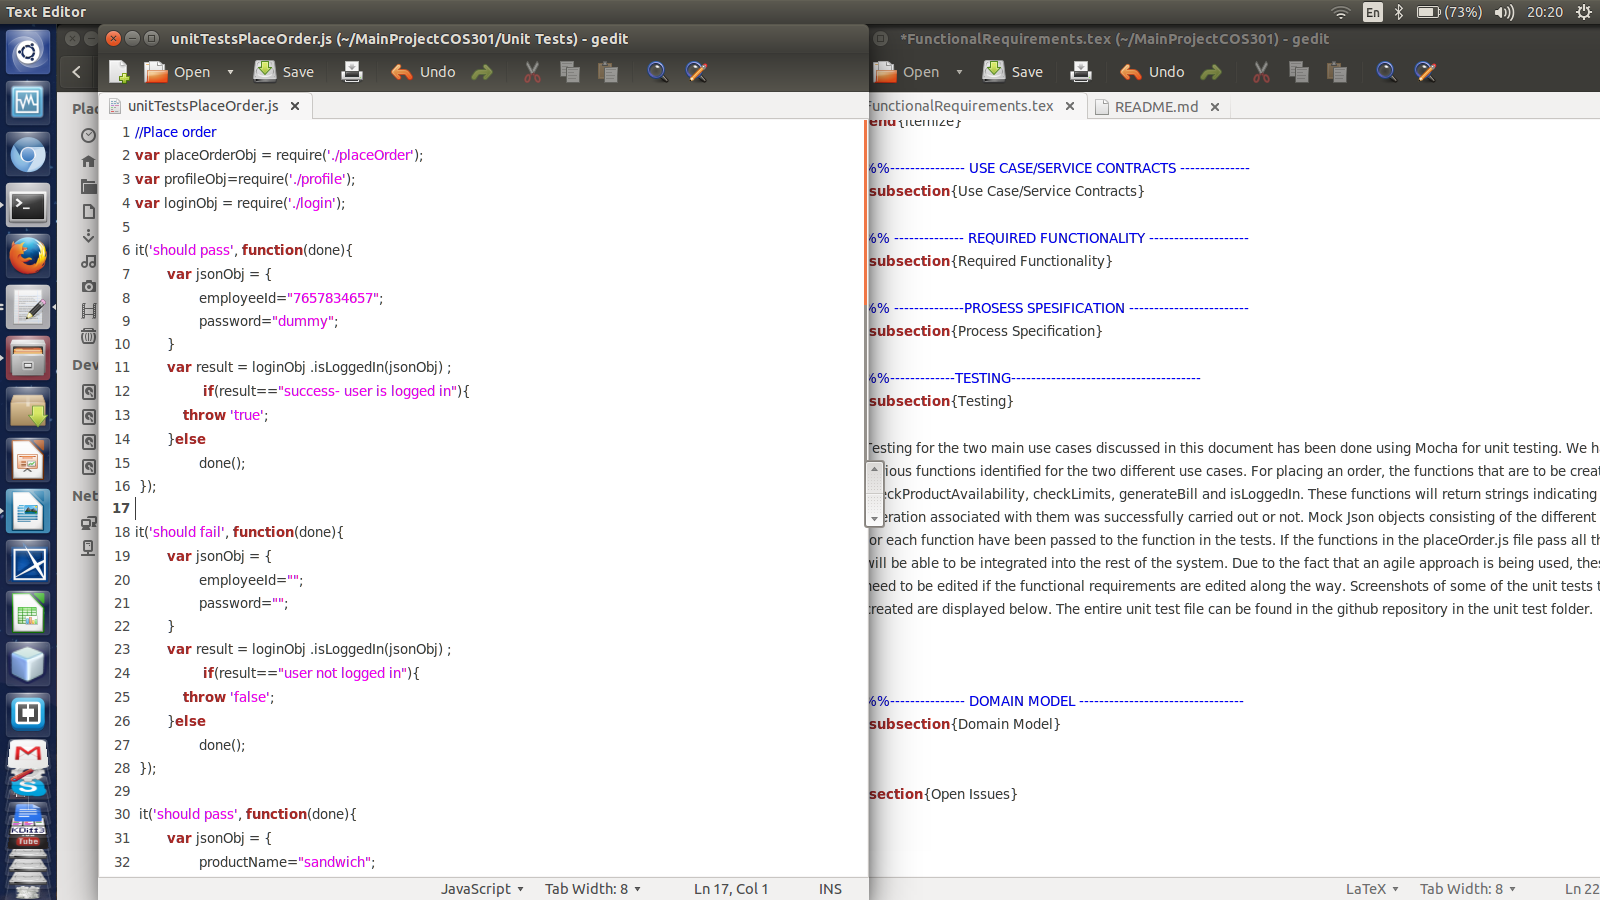
\includegraphics[width=0.85\textwidth]{placeOrderPic} 
\end{figure}
\begin{figure}[h!]
  \centering
    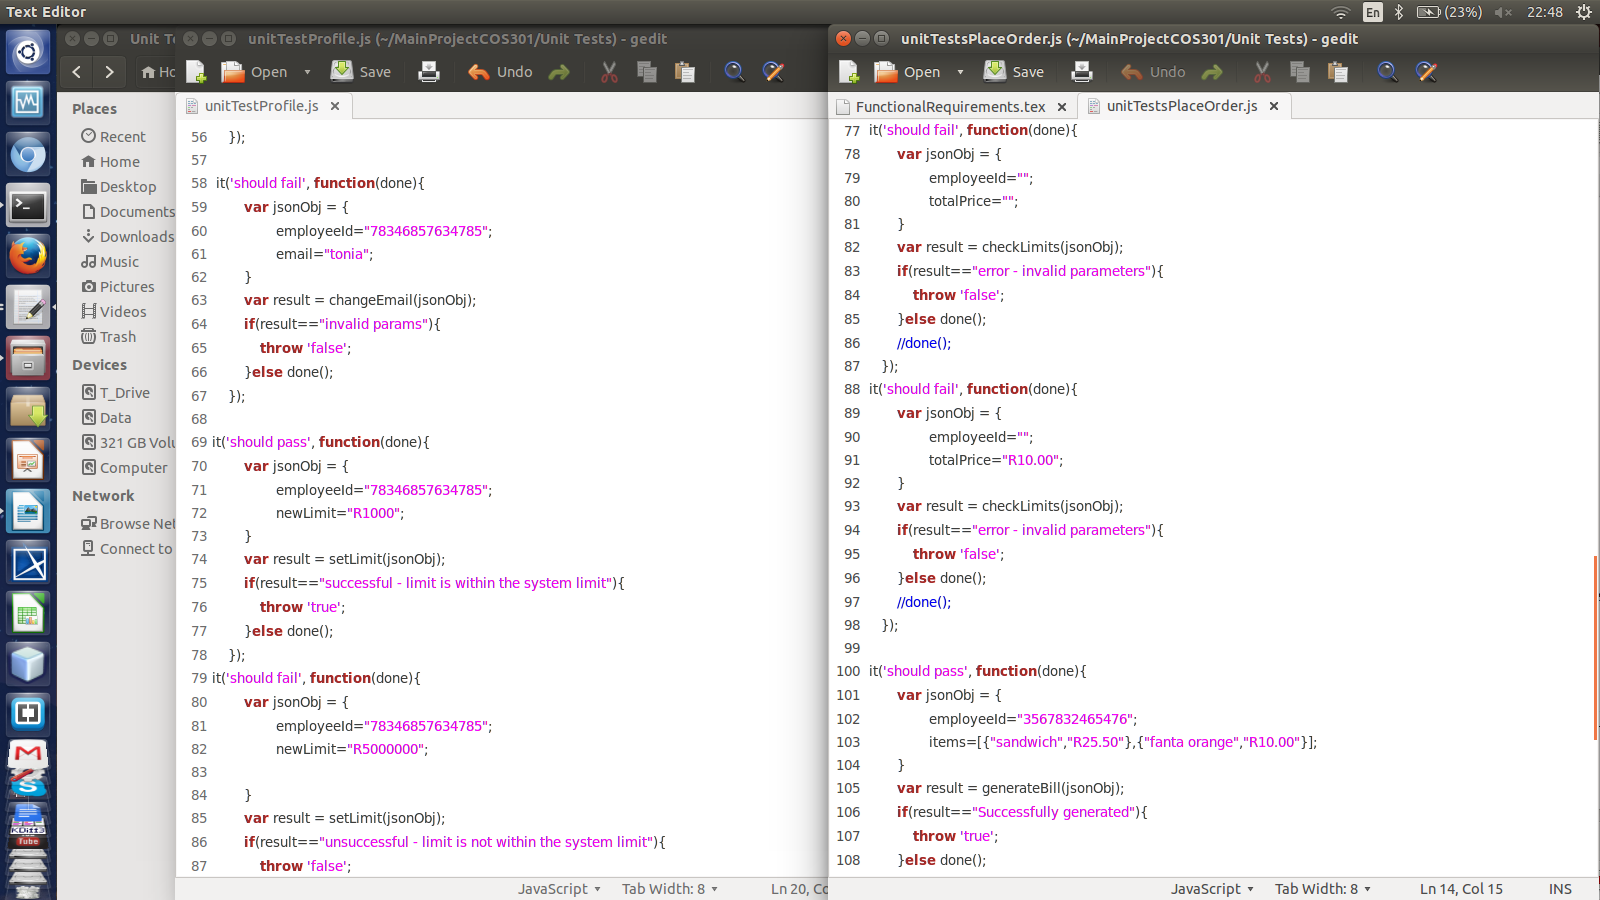
\includegraphics[width=0.85\textwidth]{placeOrder2} 
\end{figure}
\\
The second use case is manage profile, and the functions that have thus far been identified for this use case are editProfile, changePassword, changeEmail, setLimit, editRecipients, displayBill, viewHistory and generateFavourites. 
\\
The system must hence allow the logged in user to change their various settings, as well as allow the user to view the day's bill as well as the account history.
\\
A sample of the code from the unit testing file is displayed below.
\begin{figure}[h!]
  \centering
    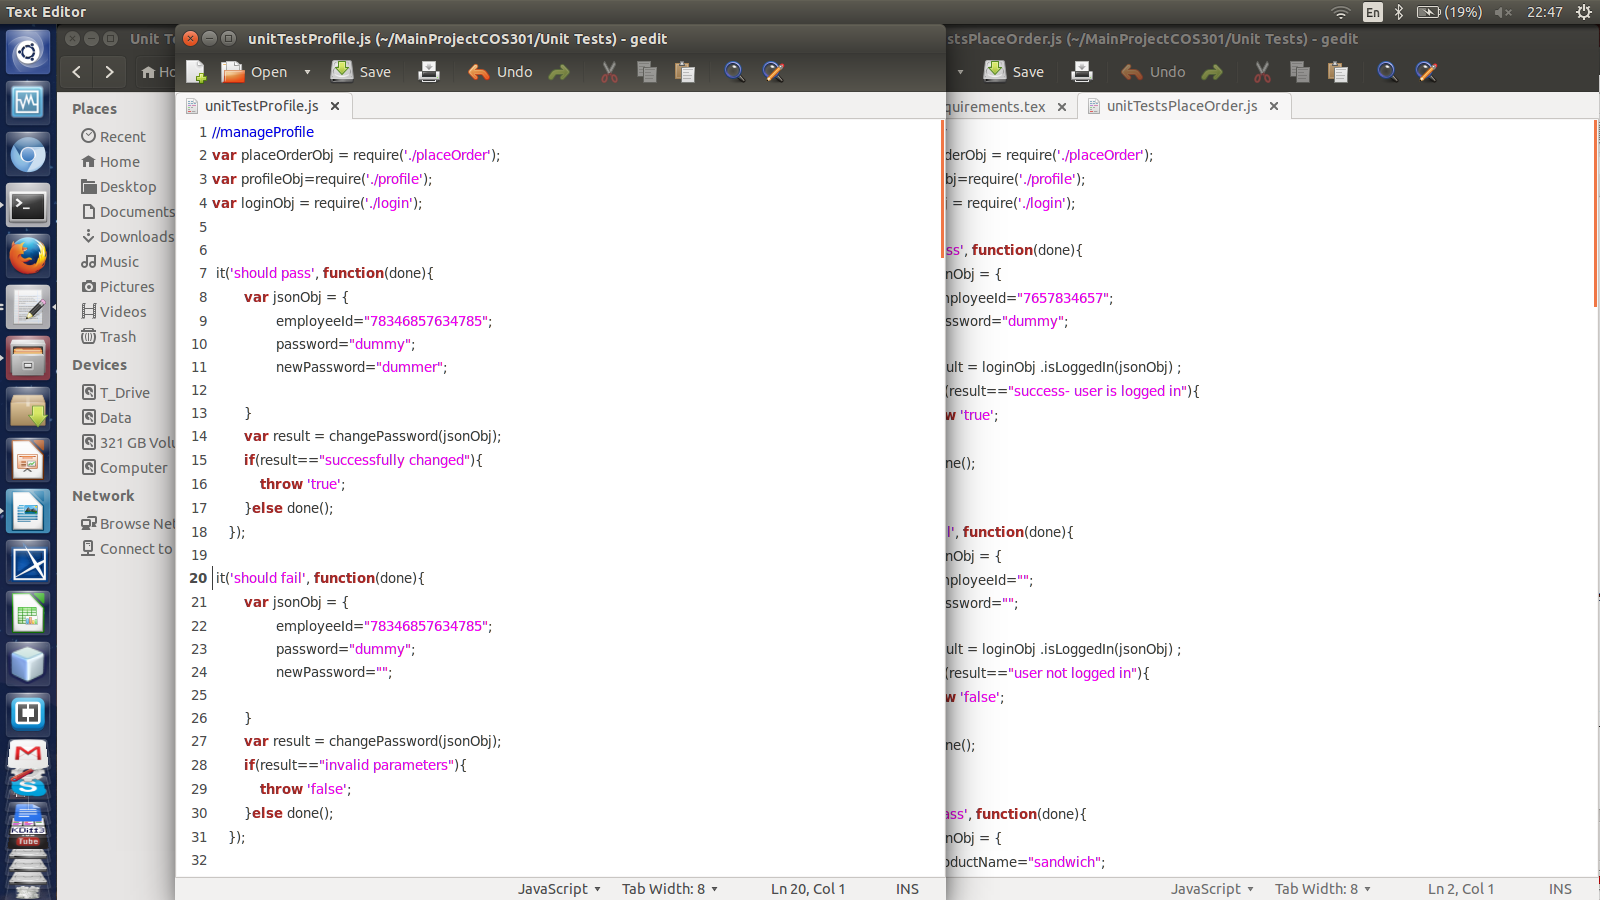
\includegraphics[width=0.85\textwidth]{profilePic} 
\end{figure}
\begin{figure}[h!]
  \centering
    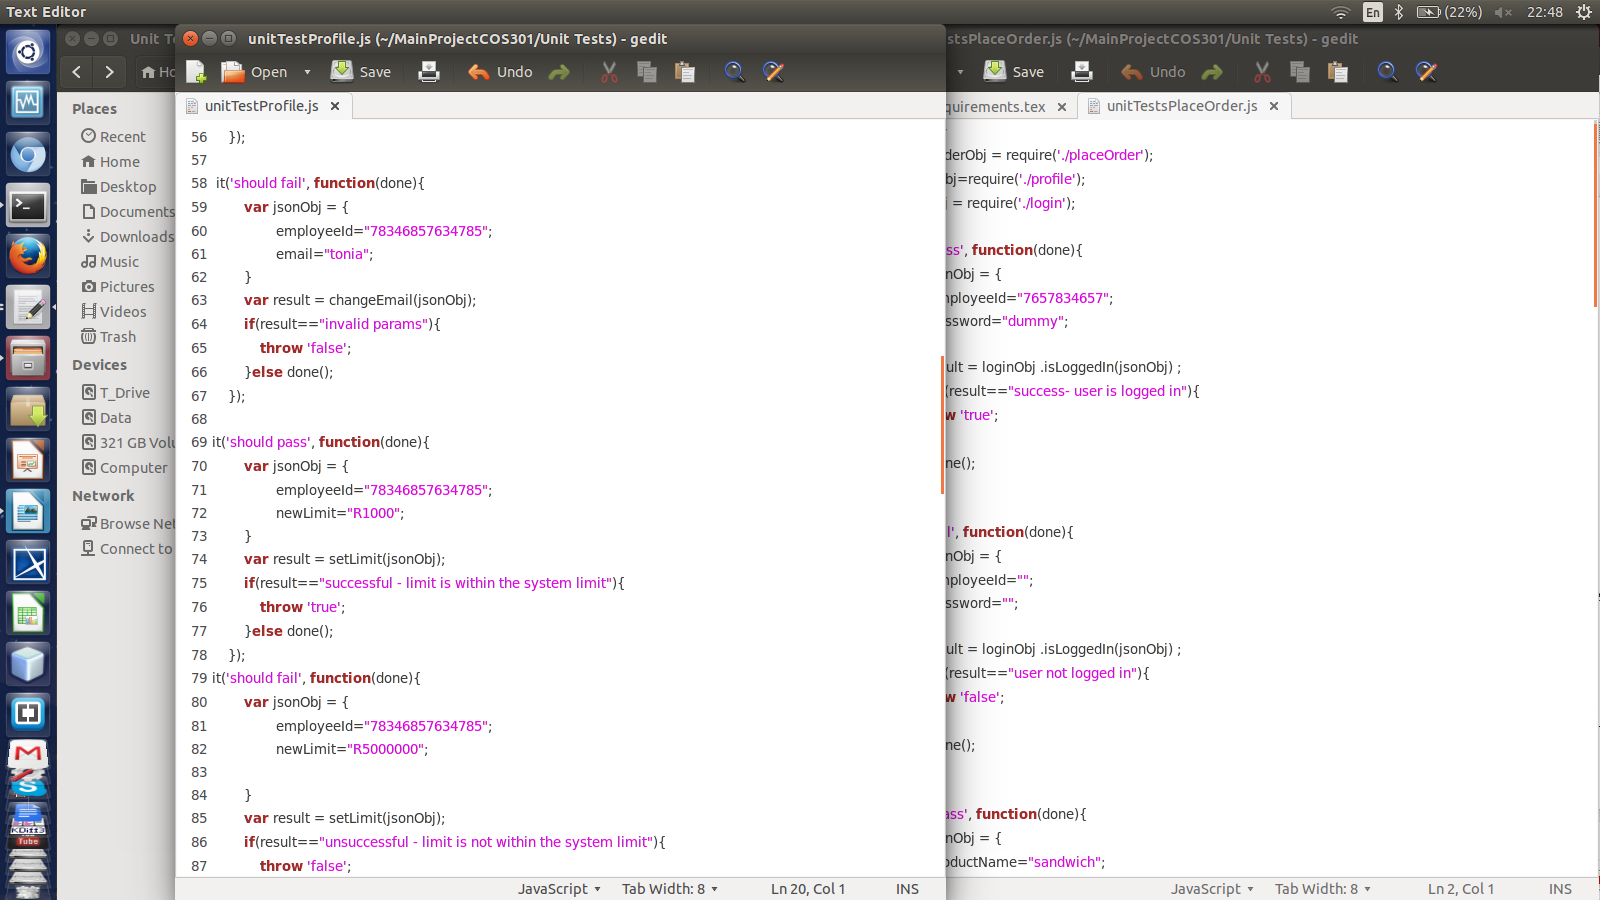
\includegraphics[width=0.85\textwidth]{profile2} 
\end{figure}

%%--------------- DOMAIN MODEL ---------------------------------
\subsection{Domain Model}


\section{Open Issues}








\end{document}

